\subsubsection{Overview of the desktop client}
The \term{UML} diagram in \refer{fig:des_uml-overview} describes the whole desktop client.
\begin{figure}[htb!]
%	\addScaledImageVertical{0.172}{des_UML.jpeg}
	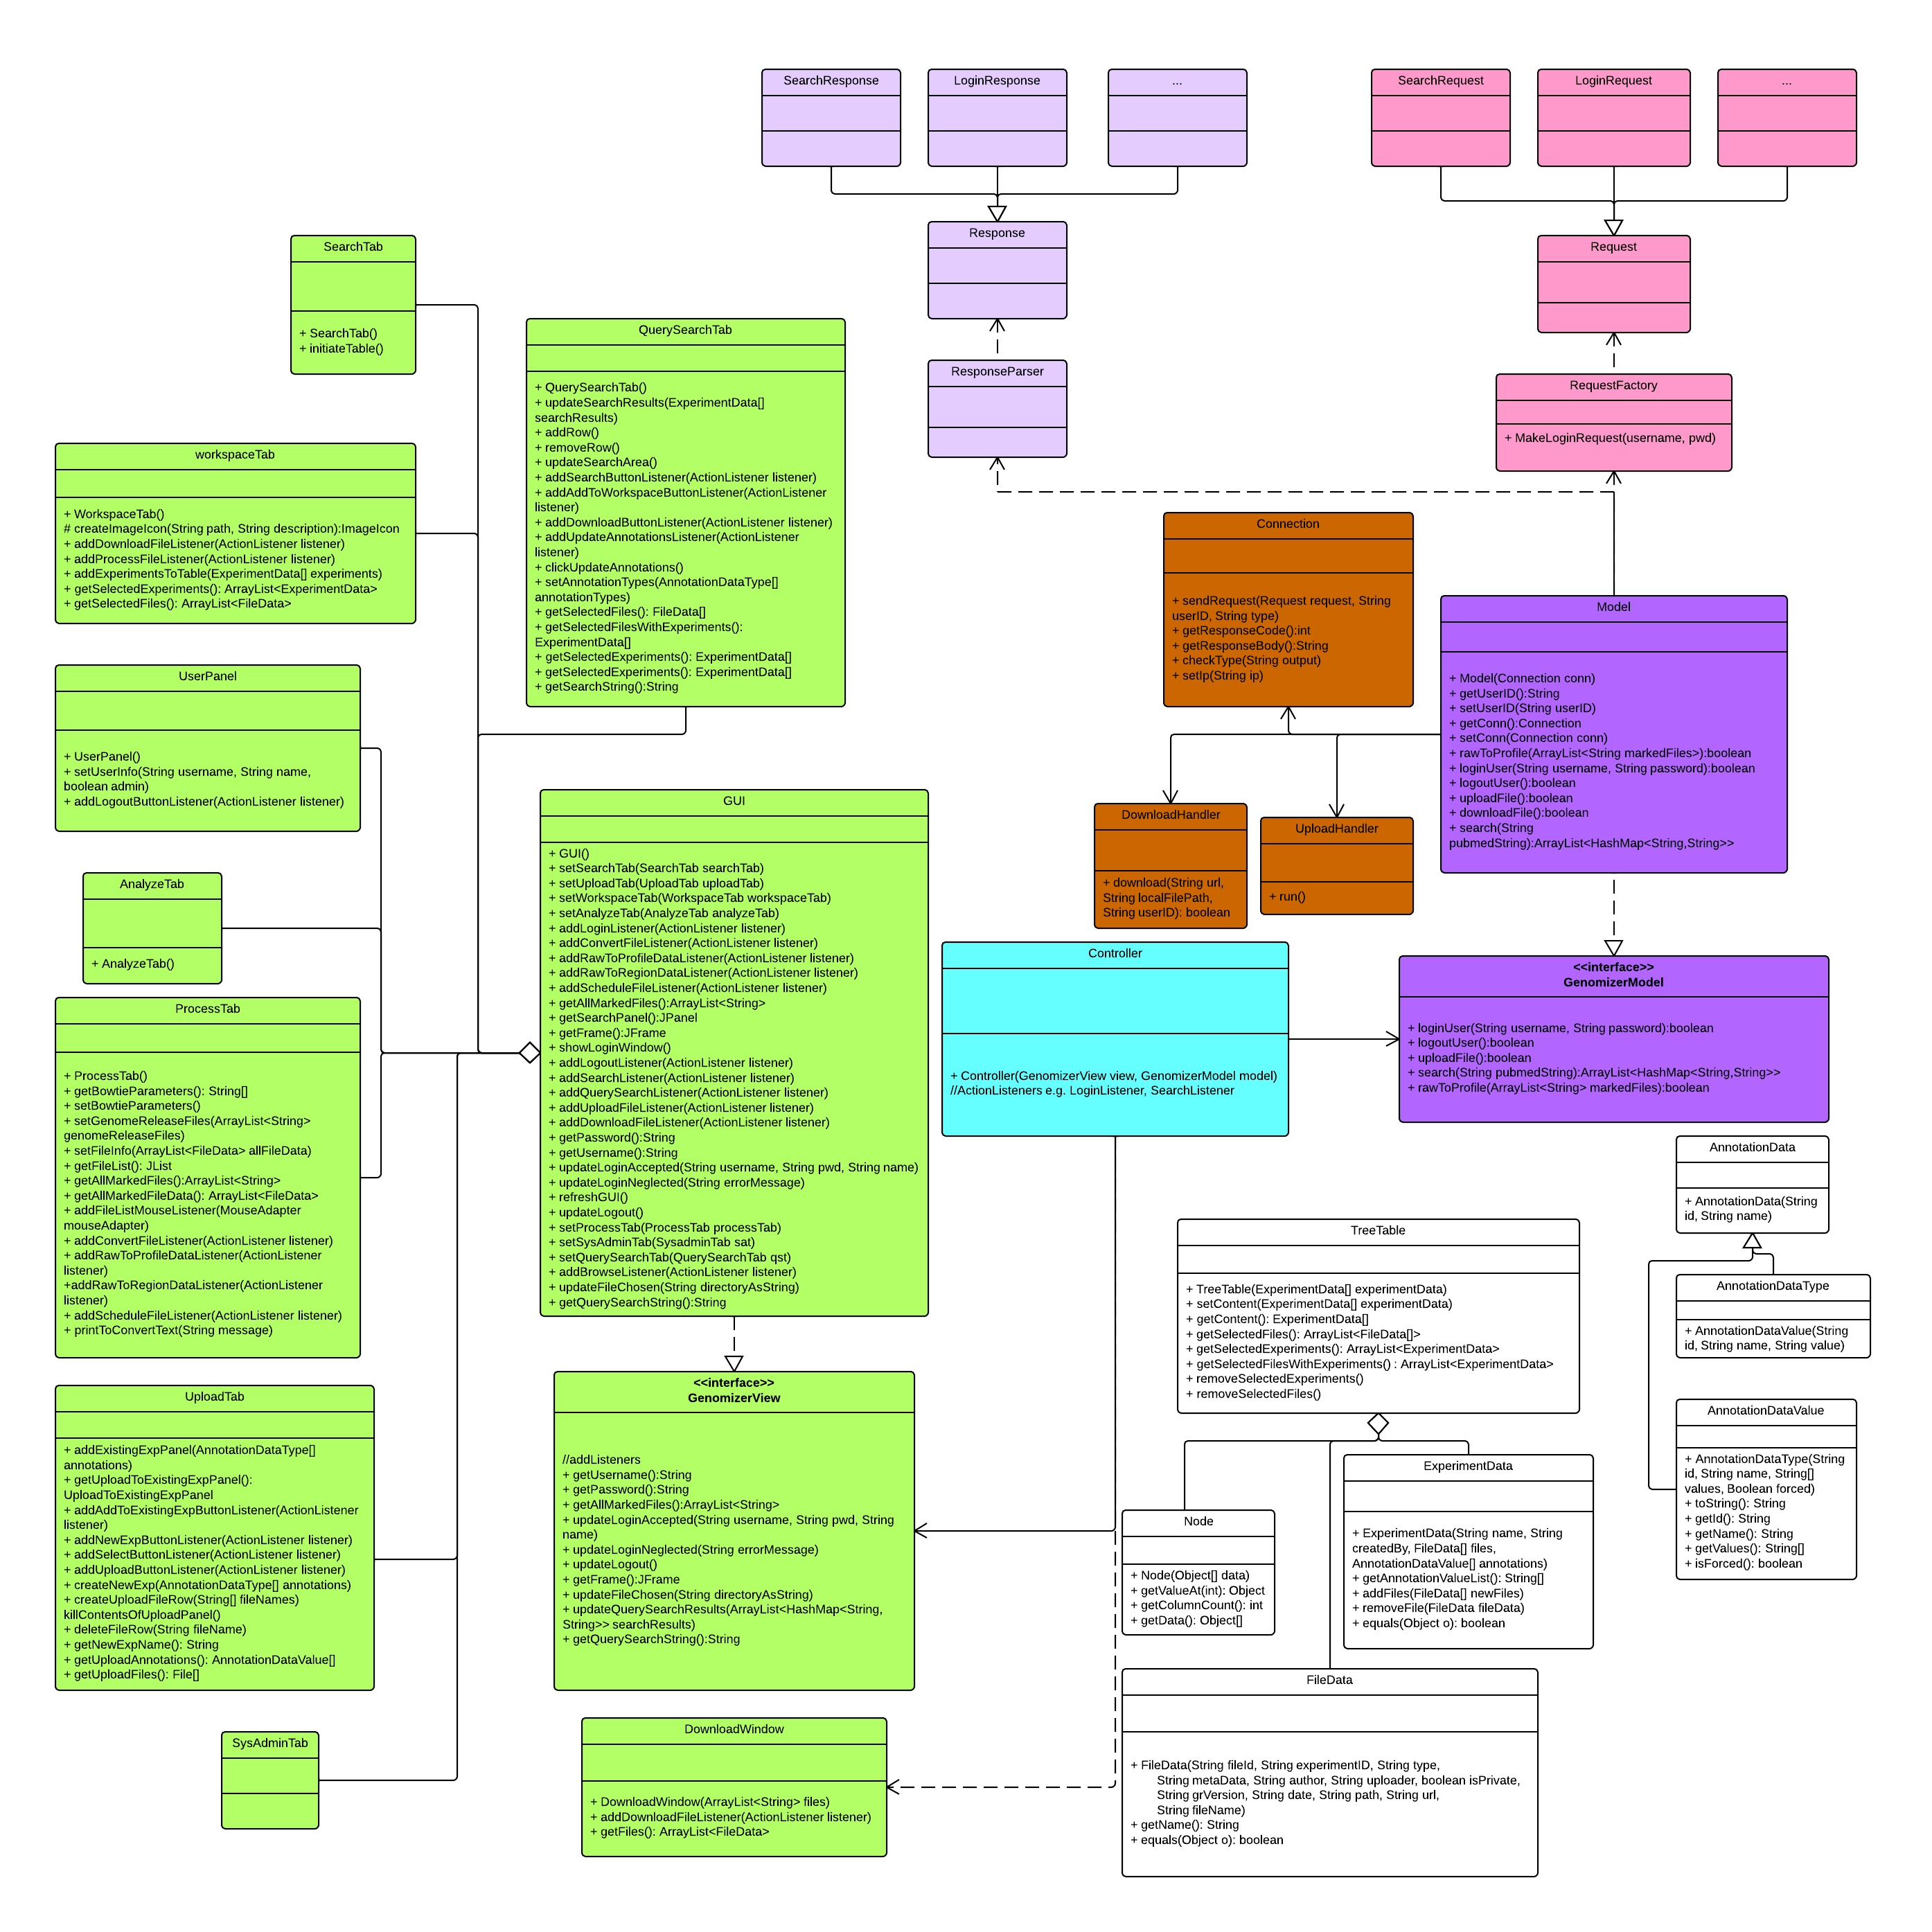
\includegraphics[width=\textheight,height=\textwidth, angle=90]{des_UML.jpeg}
	\caption{UML diagram over the desktop client}
	\label{fig:des_uml-overview}
\end{figure}

\subsubsection{View}
The view of the \appName\ Desktop client is constructed around tabs. There are 6 different tabs. These are \term{Search}, \term{Process}, \term{Upload}, \term{Workspace}, \term{Analyse} and \term{Administration}. In this version the \term{Analyze} tab is not used.

Each tab in the view is represented by its own java class. The \term{QuerySearchTab} class which represents the search tab can display both a search view and a results view. It uses the \term{QueryBuilderRow} class to construct the rows in the query builder which is used to construct search queries. The \term{QueryBuilderRow} class represents a row in the query builder and each row is dynamic and can change accordingly to user interaction.

The \term{UploadTab Class} represents the upload view of the \term{GUI}. It has functionality to both upload a file to an existing experiment (which is separately handled in the UploadExistingExpPanel) and to create a new experiment to upload files to.

The \term{ProcessTab} class represents the process view in the \term{GUI}. It contains a list where files to be processed can be stored and buttons and eight parameters for initiating the processing.

The \term{WorkspaceTab} class consists of six buttons and a \term{TreeTable} that holds all the experiments and their data. The buttons are: Delete from database, Remove selected, Download selected, Analyze selected, Browse local files and Process selected. From the workspace, the download function/window is accessible. The \term{DownloadWindow} holds the \term{FileData} to be downloaded and its \term{GUI} consists of a \term{JTable} showing the file names and has JComboBoxes for choosing file format and a download button which opens a JFileChooser to download files.

The \term{AnalyzeTab} Class is not yet implemented.

\subsubsection{Model}
The model part of the system contains method for doing most of the logic in the system. For example there are methods for sending login requests and for downloading files. There are separate classes for downloading and uploading files as well as a class for regular communication with the server called \term{Connection}.

\subsubsection{Requests}
The \term{Request} package contains the \term{Request} class , the \term{RequestFactory} and all the classes that extends the \term{Request} class. \term{Request} is the super class and can make a \term{JSON} package that all the other \term{Request} classes can use. All requests must have a name, type and an \term{URL}, but can consist of more information. For example \term{LoginRequest} also has username and password. \term{RequestFactory} is a class that can create all objects from all types of requests. It is a way to easily create all requests from the same place.


\subsubsection{Response}
This package consists of all types of responses that the server can send to the client-program. There is a class named \term{Response} that all the other response classes extends from. For example there is \term{LoginResponse}, \term{SearchResponse}. All these types of responses has different properties. There is also a class \term{ResponseParser} that can parse the responses so that the important information can be taken out of a \term{JSON}-package. This information can then be used to tell the client program what should happen next in the user interface. 


\subsubsection{Controller}
The controller part of the system consists of \term{ActionListeners} for the different buttons and functionalities in the view. For example there are Listeners for searching, downloading and processing. The Controller class has access to both the view and the model and acts as a middle hand between those two parts of the system. Usually a Listener in the controller reacts upon user input and then modifies the model and gives information about the change to the view.
\FloatBarrier

\subsubsection{Utilites}

There are several classes which represents different data in the system. There are classes for experiment data, file data and annotation data. For example when a search response is received from the server it is parsed into experiment data and the experiment data contains file data and annotation data.

The TreeTable class represents the table which displays experiment data, annotation data and file data in the Search and Workspace tabs. It is specially constructed to handle the data classes and it allows vertical sorting.

\subsubsection{System Administration}
%Till Anna!
The System Administration Tab is developed separeately from the rest of the Desktop GUI, and hence has it's own back end description here. 

\paragraph{Observer observable}
\label{Observer observable}

\begin{figure}[htb!]
\addImage{des_sysadminUML.png}
\caption{Communication UML}
\label{fig:adm_viewmodelcomuml}
\end{figure}

Observer is an interface and Observer is a class, and together they are used to simplify communication. This pattern is used when one object needs to be automatically notified of changes in another object. The observing object has to implement the Observer interface. This interface enforces only the \textit{update()} method which will be triggered every time something changes in the observed object. The Observable on the other hand is a class and any object that wants to be observed has to extend the Observable class. The Observable class has a few methods that can be of use but most important ones are \textit{addObserver()}, which is used to add an observer that will observe this object, \textit{setChanged()} simply sets flag that verifies that this object has changed, and finally \textit{notifyObservers()} that notifies all objects observing this object that something has changed and so triggers their \textit{update()} methods.

This pattern is used for communications between the system administration view and the main controller.

\paragraph{View to controller communication}


When the user requests a state change on the server of any kind, the following steps occur. When the user clicks the button to trigger the request a listener will fetch the data from the GUI and package it into a specific datatype. When finished the listener triggers the \textit{notifyObservers(<object>)} method with the datatype as an argument. Which in turn triggers the \textit{update()} method in the \textit{SendDataObserver} class located in the main controller. The \textit{SendDataObserver} unpacks the data and then calls the model which creates the request.

In \refer{fig:adm_viewmodelcomuml} an example of this communication flow is visible. An example is when a user wants to create a new annotation. Once the user has filled in all the neccesary fields in the new annotations view, the user clicks the 'Create annotation' button (See \refer{fig:adm_desktopgui}). The \textit{AnnotationPopupListener} receives the event and calls the \textit{sendNewAnnotation()} method in the \textit{SysadminController} class. This method then creates an instance of the datatype \textit{AddAnnotationRequest} using the input from the textfields in the \textit{SysadminAnnotationPopup}. Since the  \textit{SysadminController} is an Observable object, it then uses the inherited methods \textit{setChanged()} and \textit{notifyObservers()}. This triggers the \textit{update()} method in the \textit{SendDataObserver} class (which implements the Observer interface and is an inner class of the \textit{Controller} ). The \textit{update()} method only receives an object, so first it verifies that the Object is of the \textit{AddAnnotationsRequest} type, and then extracts the neccesary attributes from the datatype and sends them to the \textit{GenomizerModel} which create the request.





\subsubsection{Annotation}

The annotation tab is implemented in the class \textit{AnnotationsViewCreator} 

\paragraph{Add annotations}
When adding a new annotation which is done from the popup window that is implemented in the \textit{SysadminAnnotationPopup} class, the \textit{AnnotationPopupListener} recives an event. The event is parsed and the \textit{sendNewAnnotation()} method will be executed in the \textit{SysadminController} class. Here the input from the user will be fetched and sent into a new datatype object of \textit{AddAnnotationRequest} (located in the \textit{requests} packet). This object will in turn be sent to the model via the observer observable (see \ref{Observer observable} - Observer observable) design pattern that is implemented. 



\subsubsection{Flow of the system}

The sequence diagram in \refer{fig:des_download-sequence} describes the flow of the system when the user presses the download file button and the diagram in \refer{fig:des_login-sequence} describes how the desktop clients reacts to a login.





\begin{figure}[htb!]
	\addImage{des_downloadsequence.jpeg}
	\caption{UML sequence diagram of downloading a file}
	\label{fig:des_download-sequence}
\end{figure}

\begin{figure}[htb!]
	\addImage{des_loginsequence.jpeg}
	\caption{UML sequence diagram of login}
	\label{fig:des_login-sequence}
\end{figure}
\FloatBarrier
